\documentclass[11pt]{article}
\usepackage[margin=1in]{geometry}
\usepackage[T1]{fontenc}
\usepackage{lmodern}
\usepackage{amsmath}
\usepackage{booktabs}
\usepackage{graphicx}
\usepackage{xcolor}
\usepackage[hidelinks]{hyperref}
\usepackage{url}

\graphicspath{{../benchmarks/results/}{../docs/img/how/}}

\title{Fused Attack Graphs for Budgeted Remediation:\\
An Open Evaluation of LINCHPIN with a Measured Lab}
\author{Rakshit\\VIT Chennai}
\date{Preprint, October 2026 \quad (not peer reviewed)}

\begin{document}
\maketitle

\begin{abstract}
Vulnerability management usually ranks findings one at a time, by CVSS, EPSS or membership in CISA's Known
Exploited Vulnerabilities (KEV) catalog. Choosing a minimum set of fixes that disconnects an attack graph is a
classical alternative, but open, reproducible evidence about \emph{which data} such plans need is scarce. We present
LINCHPIN, an open-source, read-only tool that fuses already-collected scanner exports, Active Directory identity data
and network segmentation into one attack graph with exploit-intelligence edge costs, and recommends a budgeted,
evidence-carrying set of fixes: the exact minimum vertex cut when it fits the budget, a greedy set cover otherwise.
On seeded synthetic topologies with real CVE parameters, and inside LINCHPIN's own model, identity data decides
whether three fixes suffice where routes run through cached credentials: 100 of 100 such topologies are disconnected
with it and 5 [2, 11] without it (paired exact McNemar $p < 10^{-4}$). Over the 150 topologies where a three-fix cut
exists, the exact budgeted interdiction program of Israeli and Wood also reaches 100\%, a greedy interdiction
heuristic 97\% [92, 99] and the best patch-only plan 95\% [90, 97], while score-sorted patch queues restricted to
on-path vulnerabilities reach 9--10\%, no better than three remediable nodes drawn at random. In a lab of five
deliberately outdated container images scanned inside continuous integration, one upgrade disconnects the database
(as do betweenness and both interdiction baselines) while a CVSS-first queue needs three. A partial replication of a
published EPSS-versus-CVSS comparison with public labels matches its effort figures within two points; on a
prospective label EPSS covers 33 and CVSS 18 of the same 62 exploited CVEs at equal effort ($p = 0.004$). Code, data
pointers and every result, with the commit or CI run that produced it, are public.
\end{abstract}

\section{Introduction}

A remediation queue sorted by CVSS treats a critical vulnerability on an unreachable host as urgent and two moderate
ones that chain to the domain controller as routine. Exploit prediction (EPSS~\cite{jacobs2021epss}) and the KEV
catalog sharpen the per-finding signal, but they still score findings in isolation. Attack graphs~\cite{phillips1998graph,sheyner2002automated,ou2005mulval}
model how an attacker chains footholds, and minimum-cost hardening~\cite{noel2003efficient,wang2006minimum,albanese2012time}
and budgeted blocking of identity graphs~\cite{dunagan2009heatray,guo2022practical,guo2023scalable} turn them into fix
plans. The algorithmic core of such planning is well studied. What practitioners lack is open evidence about the
inputs: how much does a plan depend on identity data, on segmentation, on exploit intelligence, and how does it compare
with published planners and with the score-sorted queues that are actually used?

This paper does not propose a new cut algorithm; LINCHPIN's cut is a vertex max-flow~\cite{ford1956maximal}. Its
contributions are:
\begin{itemize}
  \item an open, read-only system that fuses real exports (OpenVAS, Nessus, nmap, SharpHound and a topology overlay)
        with public exploit intelligence (NVD, EPSS, KEV) into one deterministic attack graph and returns fix plans in
        which every fix carries a templated rationale and the paths it breaks (Section~\ref{sec:system});
  \item a seeded benchmark with ground truth and an \emph{ablation} that isolates which data makes plans work, with
        paired tests and confidence intervals (Sections~\ref{sec:setup}--\ref{sec:results});
  \item comparisons with published planners: the exact budgeted shortest-path interdiction program of Israeli and
        Wood~\cite{israeli2002shortest} and a greedy interdiction heuristic in the style of Guo et
        al.~\cite{guo2023scalable};
  \item a \emph{measured} case study in which continuous integration starts outdated official container images on
        isolated networks, detects their versions, and checks the resulting plan; and a partial replication of
        Jacobs et al.'s EPSS evaluation~\cite{jacobs2023enhancing} with public labels.
\end{itemize}

\section{Related work}
\label{sec:related}

\paragraph{Attack graphs and hardening.} Phillips and Swiler introduced graph-based vulnerability
analysis~\cite{phillips1998graph}; Sheyner et al.\ generated attack graphs by model checking~\cite{sheyner2002automated};
MulVAL derives them with logic programming~\cite{ou2005mulval}. Noel et al.~\cite{noel2003efficient} and Wang, Noel and
Jajodia~\cite{wang2006minimum} compute minimum-cost hardening measures, and Albanese et al.\ make it time-efficient for
large graphs~\cite{albanese2012time}. LINCHPIN's graph model is deliberately simpler than logical attack graphs: hosts,
services, vulnerabilities, privileges, credentials, AD access-control entries and data stores, with an exact vertex cut
over remediable nodes.

\paragraph{Fusing scanner and network data.} TVA~\cite{jajodia2005topological}, NetSPA~\cite{ingols2006practical} and
CyGraph~\cite{noel2016cygraph} (the latter in Neo4j) already combine vulnerability scans with firewall rules and
topology into attack graphs. LINCHPIN adds the Active Directory identity layer from SharpHound (sessions, cached
credentials, abusable access-control entries) to that fusion, together with public exploit intelligence, and evaluates
which of these inputs the plans depend on.

\paragraph{Identity graphs.} Heat-ray combats identity snowball attacks with combinatorial optimization over
credential graphs~\cite{dunagan2009heatray}. Guo et al.\ study budgeted blocking of Active Directory attack graphs with
fixed-parameter algorithms~\cite{guo2022practical} and scalable edge blocking with a greedy
baseline~\cite{guo2023scalable}. LINCHPIN ingests the same kind of SharpHound data but fuses it with vulnerability and
segmentation data.

\paragraph{Interdiction.} Shortest-path interdiction maximizes the adversary's shortest path after a budget of
removals; Israeli and Wood give a mixed-integer formulation via the dual of the inner shortest-path
problem~\cite{israeli2002shortest}. We use it as the optimal baseline when no cut fits the budget.

\paragraph{Prioritization.} EPSS predicts exploitation from public and commercial signals~\cite{jacobs2021epss}; its
third version is evaluated against CVSS and KEV in terms of coverage, efficiency and effort~\cite{jacobs2023enhancing}.
LINCHPIN uses CVSS, EPSS and KEV only inside its edge costs.

\section{System}
\label{sec:system}

\paragraph{Findings.} Connectors parse exports into one frozen schema, the \emph{normalized finding}
(kinds: \texttt{cve}, \texttt{service}, \texttt{credential}, \texttt{acl}, \texttt{config}, \texttt{reachability}),
validate it, and merge scanner host identifiers onto topology identifiers through declared aliases. When a scan only
reports product versions, an offline index of NVD's version ranges maps them to CVEs, one finding per service; the
fix is then an upgrade. Findings are enriched with the CVSS vector and exploitability sub-score, EPSS and KEV status.
LINCHPIN never contacts a host.

\paragraph{Graph.} Directed edges follow the attacker: the internet or a host reaches a service
(\texttt{CAN\_REACH}, from segment rules), a service has a vulnerability (\texttt{HAS\_VULN}), a vulnerability whose
CVSS vector implies code execution yields a privilege (\texttt{ENABLES}), a privilege controls a host
(\texttt{LEADS\_TO}), a host stores credentials (\texttt{STORED\_ON}) that grant privileges elsewhere
(\texttt{GRANTS}), abusable access-control entries grant control of principals and hosts, and a host holds a data
store. Each edge gets a deterministic cost in $[0,1]$:
\begin{equation}
c(e) = \frac{w_1 (1 - x_e) + w_2 (1 - m_e) + w_3 s_e}{w_1 + w_2 + w_3},\qquad (w_1, w_2, w_3) = (0.5, 0.3, 0.2),
\end{equation}
where $x_e$ is exploitability ($0.6$ times the normalized CVSS exploitability sub-score plus $0.4$ times EPSS, at least
$0.95$ for KEV entries, and $1$ for non-exploit edges), $m_e$ is a prerequisite match ($0.5$ for credential use whose
target is not reachable from where the credential is stored, $1$ otherwise), and $s_e$ is a skill penalty per
transition class.

\paragraph{Paths, cuts, plans.} Paths from entry points to crown jewels are enumerated with Yen's
algorithm~\cite{yen1971finding} on the subgraph that is both reachable from an entry and able to reach a crown jewel.
\emph{Chokepoints} come from the dominator tree of a virtual source; the \emph{minimum remediation cut} from a
vertex-split max-flow over remediable nodes (vulnerabilities, credentials, access-control entries and non-entry
hosts). The plan uses the exact cut whenever it fits the budget, ordered by a greedy set cover of the enumerated paths;
otherwise the greedy set cover alone. Every fix carries a rationale from templates (no language model) and the
identifiers of the enumerated paths it breaks. A what-if query recomputes paths with nodes removed.

\section{Evaluation setup}
\label{sec:setup}

\paragraph{Topologies.} Four families with 50 seeds each and $12 + (\text{seed} \bmod 49)$ hosts (58 to 317 graph
nodes): \texttt{single} (one bastion; minimum cut 1), \texttt{multi} (parallel bastions and two routes into the
database, one through a cached credential; cut 2, no chokepoint), \texttt{none} (flat network; cut about 7, larger than
the budget) and \texttt{ad} (tiered Active Directory with cached administrator sessions; mean cut 1.34). Every
vulnerability uses the CVSS vector, sub-score, EPSS and KEV status of a real CVE from a stratified sample of 3,000
(10\% KEV, against about 0.5\% in the source population). Every topology also contains two unreachable hosts with
KEV-listed critical vulnerabilities and high-CVSS vulnerabilities without code execution: distractors for
score-sorted queues.

\paragraph{Planners and metrics.} With a budget of three fixes we compare LINCHPIN, its greedy set cover alone, the
exact interdiction program~\cite{israeli2002shortest} solved with HiGHS~\cite{huangfu2018highs}, a greedy interdiction
heuristic (repeatedly remove the node on the cheapest path whose removal raises its cost most), the best patch-only
plan (LINCHPIN's planner restricted to vulnerabilities), CVSS-, EPSS- and KEV-then-EPSS-sorted queues over all
vulnerabilities and over vulnerabilities on some entry-to-crown-jewel route only, betweenness centrality, and three
nodes drawn uniformly from all remediable nodes. The queues may only patch, while LINCHPIN may also segment a host or
rotate a credential; the patch-only plan is the like-for-like ceiling for the queues. A plan \emph{disconnects} if no
crown jewel stays reachable. Where nothing disconnects we report the rise in the attacker's cheapest-path cost and its
share of the optimum. Rates carry 95\% Wilson intervals~\cite{wilson1927probable}, means seeded percentile-bootstrap
intervals~\cite{efron1979bootstrap}, paired disconnect outcomes exact McNemar tests~\cite{mcnemar1947note}, and paired
cost gains a bootstrap interval of the mean difference and an exact sign test. Graph algorithms use
NetworkX~\cite{hagberg2008networkx}.

\paragraph{Ablation.} The same optimizer plans on a degraded view of the findings and the plan is scored on the full
graph: without identity findings, with 10/25/50\% of them dropped at random, with a flat network, with every CVE
treated as code execution, with uniform edge costs, and with identity data only.

\paragraph{What the 100\% means.} LINCHPIN plans on the graph it is scored on and returns the exact cut whenever that
cut fits the budget, so it disconnects every topology where a three-fix cut exists \emph{by construction}. The
benchmark measures how far other planners fall short of that optimum inside the model; the ablation measures what
incomplete data costs. Neither measures real-world risk.

\paragraph{Provenance.} The benchmark and ablation tables were regenerated by a manual CI workflow (run 37089520295,
Linux); every outcome cell equals the earlier run on Windows. Each result file records the commit or CI run that
produced it.

\section{Results}
\label{sec:results}

\paragraph{Benchmark.} Table~\ref{tab:bench} pools the 150 topologies of \texttt{single}, \texttt{multi} and
\texttt{ad}. Score-sorted queues disconnect 3--4\% of them; restricting them to on-path vulnerabilities, which removes
the planted distractors, raises this only to 9--10\%, the same as a uniformly random choice of three remediable nodes
(10 vs 10 and 9 vs 10 discordant topologies, $p = 1$). The best patch-only plan reaches 95\%, so the queues' shortfall
is not explained by their smaller action space. Betweenness reaches 39\% (84\% on \texttt{single}, 2\% on
\texttt{multi}). The exact interdiction program also reaches 100\%, confirming that the cut itself is not the
contribution; the greedy interdiction heuristic misses five \texttt{multi} topologies. The difference in the share of
enumerated (k-capped) attack paths left after three fixes, CVSS-first minus LINCHPIN, is 92.3 points [87.8, 96.0] over
the 150 topologies (\texttt{ad} 80.9, \texttt{multi} 98.0, \texttt{single} 98.0); on \texttt{none} both leave the
capped enumeration full. Figure~\ref{fig:bench} shows the per-family rates.

\begin{table}[t]
\centering\small
\begin{tabular}{lrrr}
\toprule
planner & disconnected & 95\% interval & McNemar $p$ vs.\ LINCHPIN \\
\midrule
LINCHPIN (exact cut, else greedy) & 150/150 & [97.5, 100] & -- \\
Exact interdiction MILP~\cite{israeli2002shortest} & 150/150 & [97.5, 100] & 1 \\
LINCHPIN, greedy set cover only & 147/150 & [94.3, 99.3] & 0.25 \\
Greedy interdiction (Guo-style) & 145/150 & [92.4, 98.6] & 0.0625 \\
Best patch-only plan & 142/150 & [89.8, 97.3] & 0.0078 \\
Betweenness & 58/150 & [31.2, 46.7] & $<10^{-4}$ \\
CVSS-first, on-path only & 15/150 & [6.2, 15.8] & $<10^{-4}$ \\
Random & 15/150 & [6.2, 15.8] & $<10^{-4}$ \\
KEV then EPSS, on-path only & 14/150 & [5.6, 15.1] & $<10^{-4}$ \\
CVSS-first & 6/150 & [1.8, 8.5] & $<10^{-4}$ \\
KEV then EPSS & 4/150 & [1.0, 6.7] & $<10^{-4}$ \\
\bottomrule
\end{tabular}
\caption{Disconnection with a budget of three fixes, pooled over the \texttt{single}, \texttt{multi} and \texttt{ad}
families (50 seeds each). Patch-only: LINCHPIN restricted to vulnerabilities; random: three remediable nodes
drawn uniformly.}
\label{tab:bench}
\end{table}

\begin{figure}[t]
\centering
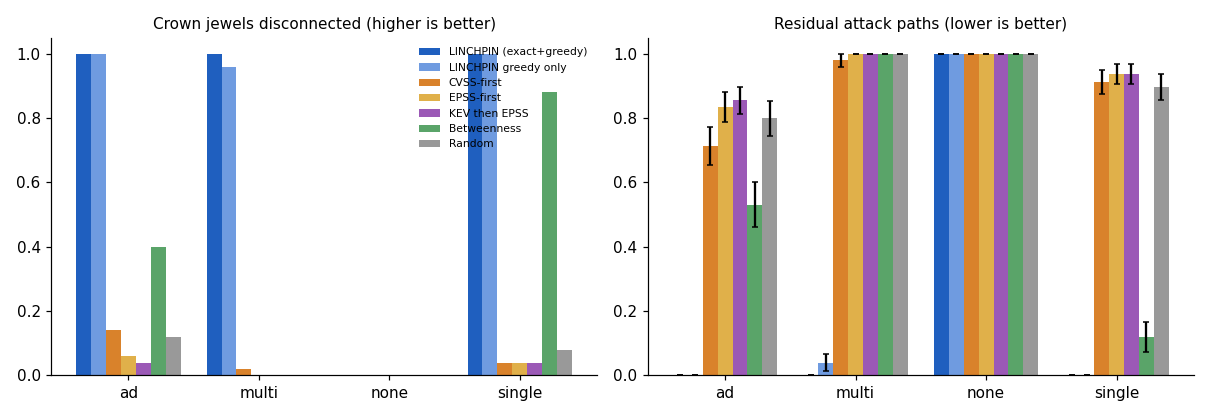
\includegraphics[width=\linewidth]{strategies.png}
\caption{Disconnect rate (left, 95\% Wilson intervals) and attack paths left (right, mean $\pm$ s.e.) per family.}
\label{fig:bench}
\end{figure}

\paragraph{No cut within budget.} On \texttt{none} nothing can be disconnected with three fixes. The exact program
raises the attacker's cheapest-path cost by $+0.227$ [0.209, 0.245] edge-cost units on average; LINCHPIN's greedy
fallback by $+0.193$ [0.169, 0.216], or 0.83 [0.77, 0.88] of the optimum; greedy interdiction by 0.82 [0.75, 0.89],
KEV-then-EPSS by 0.15 [0.09, 0.22] and CVSS-first by 0.09 [0.04, 0.15] of it. Paired on the same topologies,
LINCHPIN's gain exceeds KEV-then-EPSS's by $+0.156$ [0.130, 0.182] (larger in 46 of 50, smaller in none; sign test
$p < 10^{-4}$). Using the exact program as the fallback is an obvious next step.

\paragraph{Ablation.} Table~\ref{tab:ablation} shows the planner's dependence on identity data. In the two families
whose routes run through cached credentials (\texttt{ad} and \texttt{multi}, by construction of the generator), the
fused planner disconnects 100 of 100 topologies [96.3, 100], the planner without identity findings 5 [2.2, 11.2]
(95 vs 0 discordant, $p < 10^{-4}$) and identity data alone 27 [19.3, 36.4]; in \texttt{single} identity data does
not matter. The pooled 37\% therefore reflects the family mix, not a population rate. Dropping 25\% or 50\% of the
identity findings lowers the pooled rate to 95.3\% and 90.0\%. On real data (public OpenVAS, Nessus, nmap and
SharpHound sample reports placed into a declared topology; one topology), the planner without identity findings sees
no attack path at all and proposes nothing, while the domain controller stays reachable; the fused plan's one
credential rotation cuts it off.
Over-approximating views still disconnect (a cut of a super-graph cuts the real graph) but need more fixes: a flat
network 1.82$\times$ [1.72, 1.92] the optimum on \texttt{single}, treating every CVE as code execution 1.10$\times$
[1.02, 1.20] on \texttt{ad}; greedy alone needs 1.22$\times$ [1.14, 1.31] on \texttt{multi}. Uniform edge costs leave
cuts unchanged and re-rank paths (Kendall's $\tau$ 0.36--0.51 against the intelligence-based costs). Their effect on
the cost gain depends on how plans are scored: with the intelligence-based costs the fused plan's gain on
\texttt{none} exceeds the uniform-cost plan's by $+0.144$ [0.119, 0.168] (46 vs 3 topologies, $p < 10^{-4}$), but
with uniform scoring costs it falls short by $0.054$ [0.027, 0.082] (4 vs 20, $p = 0.0015$). The ablation therefore
does not show that exploit intelligence improves plans against a real attacker.

\begin{table}[t]
\centering\small
\resizebox{\linewidth}{!}{%
\begin{tabular}{lrrr}
\toprule
planner's view of the data & disconnected (of 150) & 95\% interval & McNemar $p$ vs.\ fused \\
\midrule
fused (LINCHPIN) & 100\% & [97.5, 100] & -- \\
without the exact cut & 98.0\% & [94.3, 99.3] & 0.25 \\
10\% of identity findings dropped & 100\% & [97.5, 100] & 1 \\
25\% of identity findings dropped & 95.3\% & [90.7, 97.7] & 0.0156 \\
50\% of identity findings dropped & 90.0\% & [84.2, 93.8] & $<10^{-4}$ \\
without identity data & 36.7\% & [29.4, 44.6] & $<10^{-4}$ \\
identity data only & 18.0\% & [12.7, 24.9] & $<10^{-4}$ \\
no graph: KEV then EPSS & 2.7\% & [1.0, 6.7] & $<10^{-4}$ \\
flat network / every CVE as RCE / uniform costs & 100\% & [97.5, 100] & 1 \\
\bottomrule
\end{tabular}}
\caption{Ablation: each planner runs the same optimizer on a degraded view and is scored on the full graph. Pooled
over \texttt{single}, \texttt{multi} and \texttt{ad}; identity data can only matter in \texttt{ad} and \texttt{multi}.}
\label{tab:ablation}
\end{table}

\paragraph{Measured lab.} A continuous-integration job starts official images of httpd 2.4.49, nginx 1.16.1,
Tomcat 9.0.30, Redis 5.0.7 and MySQL 5.5.62 on two Docker networks created as internal (no route outside), and runs
version detection only (\texttt{nmap -sV}, no scripts) from a container inside each network. Segments and firewall rules
are derived from what each vantage point saw; that the first network faces the internet and that the MySQL container
holds the crown jewel are declared. Five of six services match 393 CVEs by NVD version range (7 in KEV). The minimum
cut is one fix; LINCHPIN's plan (upgrade Tomcat, the only dual-homed container) disconnects the database, as do the
interdiction planners; EPSS- and KEV-first need two fixes and CVSS-first three, because its first choice (Redis,
CVSS 9.9) lies on only half of the paths. The committed scans and analysis are the artefact of CI run 37091866743,
which also records the digest of every image it pulled.

\paragraph{A partial replication of a published comparison.} Jacobs et al.\ report coverage, efficiency and effort of
CVSS and EPSS thresholds on about 191,000 CVEs scored on 1~December 2022 against proprietary exploitation
telemetry~\cite{jacobs2023enhancing}; 73,327 of these CVEs only have CVSS~v2 in NVD, and the authors imputed their v3
vectors with their own model. We can rebuild only the 117,141 CVEs published by that date with an NVD CVSS~v3 score.
With the EPSS scores published on that date (EPSS~v2) and KEV as the public label, effort matches within two points in
all four of the paper's EPSS~v2 and CVSS rows (CVSS 7+ flags 58.2\% of CVEs, paper 58.1\%; CVSS 9.1+ 15.0\%, paper
15.1\%) and coverage within 1.5--7.5 points (CVSS 7+ covers 89.6\% [87.3, 91.5] against the paper's 82.1\%). EPSS
needs 40.8\% effort to match CVSS 7+'s coverage, an effort ratio of 0.701 [0.695, 0.824] (class-stratified bootstrap,
threshold re-matched in each replicate), against the paper's 0.671 for EPSS~v2, which lies outside the interval; at
CVSS 9.1+'s effort EPSS covers 71.4\% [68.3, 74.4] (paper: 69.9\%). The paper's headline, EPSS~v3 at one-eighth of
CVSS's effort, is not reproducible from public data because EPSS~v3 scores were not published before March 2023.
The paper documents KEV as an input feature of EPSS~v3; for v2 this is likely but not documented, so scoring EPSS
against KEV may be circular. On a prospective label (the 62 CVEs added to KEV in the following year), EPSS at CVSS
9.1+'s effort (14.9\%) covers 33 of them and CVSS 9.1+ 18: 20 against 5 discordant CVEs, exact McNemar $p = 0.0041$,
a coverage difference of $+24.2$ points with a paired bootstrap interval of [9.7, 38.7]. Efficiency does not
reproduce (1.6\% vs 8.9\%) because KEV is a much sparser label than the paper's exploitation telemetry. Every
transcribed cell of the paper's Figures 3--5 was checked against its arXiv version.

\paragraph{Learned exploitability and scale.} An optional logistic-regression model over CVE text and CVSS vectors,
trained on CVEs published 2015--2022 with KEV labels known at that date and with sentences that report exploitation
status removed, reaches ROC-AUC 0.836 [0.820, 0.852] against 0.754 [0.739, 0.772] for the CVSS base score on later
CVEs, and average precision 0.028 [0.024, 0.034] against 0.011 [0.010, 0.014]. Paired on the same bootstrap resamples,
the AUC difference is $+0.082$ [0.065, 0.100] and the average-precision ratio 2.43 [1.90, 3.24]. A first version
without these leak fixes reported 0.863 and 0.063. Building, ranking and planning take 1.1~s at 467 nodes and 7.0~s at
1,384 nodes on a laptop (median of five runs in one session); Yen's algorithm dominates. A Neo4j Graph Data Science
backend returns identical paths on graphs of up to 238,665 relationships and runs Yen 4.8--39$\times$ faster (medians of ten runs per setting in one CI run; 1.4--39$\times$ across
the four CI runs that measured it), but mirroring the graph into Neo4j costs 5--23~s.

\section{Limitations and threats to validity}

The topology families were written for this project and plans are scored inside LINCHPIN's own model, so the benchmark
measures distance from an optimum, not risk. The identity result is built into the families: only \texttt{ad} and
\texttt{multi} route through cached credentials. The exploit-intelligence ablation is scored with costs that favour
one of the two planners compared, and the order reverses with the other scoring. The score queues only patch; the
patch-only plan bounds what that restriction explains. The real-export case study uses public sample reports placed
into a declared topology; the measured lab is small and declares its internet exposure and crown jewel. Version
banners do not show backported fixes, so matched CVE lists are upper bounds. Code execution is inferred from CVSS
vectors, and Active Directory certificate services, shadow credentials, group-policy links and trusts are not
modelled. KEV is a small, curated proxy for exploitation in the wild, and the replication covers part of the paper's
population. Residual-path counts are capped at $k = 100$; disconnection and cost gain are reported for that reason.

\section{Ethics}

LINCHPIN is read-only: it parses files and sends no packets, and its output (which fixes matter most) is the same
information a defender needs. The only active probing in this work is version detection of containers that the
continuous-integration job itself starts on networks without outside routes; no exploit code was written or run, and
no third-party host was contacted. Public sample reports of deliberately vulnerable targets are used as data only.

\section{Reproducibility}

Code, the CVE pool, the CPE index, the committed scans and every result file are in the public repository
(\url{https://github.com/rakshit-737/linchpin-attack-path-analysis}); each result file records the commit or the continuous-integration run
that produced it. The downloader pins public datasets by SHA-256 and NVD's published hashes; all experiments are
seeded and deterministic (path ties do not depend on the interpreter's hash seed), and a re-run of the benchmark and
the ablation on a different operating system reproduced every outcome. The documentation lists each command with its
runtime (\url{https://rakshit-737.github.io/linchpin-attack-path-analysis/reproduce/}), and the lab, Neo4j and paper builds run in
continuous integration, which also checks that this PDF matches its source.

\section*{Acknowledgements}

The software, experiments and this manuscript were developed with substantial assistance from Claude, an AI model by
Anthropic, used for code, analysis and writing under the author's direction; the author is responsible for the
content. Data come from NIST's NVD, FIRST's EPSS, CISA's KEV catalog, and the DefectDojo and SpecterOps BloodHound
test corpora.

\bibliographystyle{plain}
\bibliography{refs}

\end{document}
